\documentclass[twocolumn]{IEEEtran}
\usepackage{graphicx}
\usepackage[utf8x]{inputenc}
\usepackage{times}
\usepackage{amssymb,amsfonts}
\usepackage[tbtags]{amsmath}
\usepackage{cite}
\usepackage{pict2e}
\usepackage{float}
\usepackage{lscape}
\usepackage[all]{xy}
\usepackage{graphics,graphicx,color,colortbl}
\usepackage{times}
\usepackage{subfigure}
\usepackage{wrapfig}
%\usepackage{multicol}
\usepackage{cite}
\usepackage{url}
\usepackage[tbtags]{amsmath}
\usepackage{amsmath,amssymb,amsfonts,amsbsy}
\usepackage{listings}
\usepackage{bm}
\usepackage{algorithm}
\usepackage{algorithmic}
\usepackage[centerlast, small]{caption}
\usepackage[colorlinks=true, citecolor=blue, linkcolor=blue, urlcolor=blue, breaklinks=true]{hyperref}
\hyphenation{ele-men-tos he-rra-mi-en-ta cons-tru-yen trans-fe-ren-ci-a pro-pu-es-tas si-mu-lar vi-sua-li-za-cion}

\begin{document}
\title{Diseño de celdas estándar en \textit{Electric}}
\author{Nicolás David Arias Sosa \textbf{Código:} $261692$ \url{ndariass@unal.edu.co}\\
	David Ricardo Martínez Hernández \textbf{Código:} $261931$ \url{drmartinezhe@unal.edu.co}\\
	Oscar Alejandro Rojas Gallego \textbf{Código:} $xxxxxx$ \url{oarojasg@unal.edu.co}\\
	Universidad Nacional de Colombia}
\markboth{}{}
\maketitle
\begin{abstract}
En la práctica de laboratorio que se describe a continuación se hizo el uso de la herramienta \textit{Electric} para la implementación de circuitos básicos y celdas estándar usando una tecnología de proceso de 500 nm. De igual modo, se hizo la implementación de un layout para resolver un problema de aplicación.
\end{abstract}
\begin{keywords}

\end{keywords}

\section{Introducción}
\subsection{Compuerta $AND$}
\noindent
La compuerta AND es una puerta lógica digital que implementa la conjunción lógica. Ésta entregará una salida \textbf{ALTA} $(1)$, dependiendo de los valores de las entradas, siendo este caso, al recibir solo valores altos en la puerta AND. Si alguna de estas entradas no son \textbf{ALTAS}, entonces se mostrará un valor de salida \textbf{BAJA} $(0)$. En otro sentido, la función de la compuerta AND efectivamente encuentra el mínimo entre dos dígitos binarios, así como la función OR encuentra al máximo.\\
Se puede ver claramente que la salida {\bf X} solamente es ``$1$'' ($1$ lógico, nivel alto) cuando la entrada {\bf A} como la entrada {\bf B} están en ``$1$''. En otras palabras la salida {\bf X} es igual a $1$ cuando la entrada {\bf A} y la entrada {\bf B} son $1$.\\
Esta situación se representa en álgebra booleana como:
\begin{equation}
 X  =  A \cdot B
 \label{ecu1}
\end{equation}

\subsection{Compuerta $NAND$}
\noindent
La puerta NAND o compuerta NAND es una puerta lógica digital que implementa la conjunción lógica negada. Cuando todas sus entradas están en ``$1$'' o en {\bf ALTA}, su salida está en $0$ o en {\bf BAJA}, mientras que cuando una sola de sus entradas o ambas están en $0$ o en {\bf BAJA}, su salida {\bf X} va a estar en $1$ o en {\bf ALTA}.\\
Se puede ver claramente que la salida {\bf X} solamente es ``$0$'' ($0$ lógico, nivel bajo) cuando la entrada {\bf A} como la entrada {\bf B} están en ``$1$''. En otras palabras la salida {\bf X} es igual a ``$0$'' cuando la entrada {\bf A} y la entrada {\bf B} son ``$1$''.\\
Esta situación se representa en álgebra booleana como:
\begin{equation}
 X = \overline {A \cdot B}  = \overline A  + \overline B
 \label{ecu2}
\end{equation}

\subsection{Flip-flop D}
\noindent


\section{Compuerta $AND$ de $3$ entradas} \label{AND3}
\noindent
La compuerta AND de $3$ entradas es la unión de $2$ compuertas AND de $2$ entradas, pero para este caso se utilizó la siguiente ecuación como las demostradas en clase.\\
Primero se utiliza la ecuación original para la parte N (ecu~\ref{ecu3}).
\begin{equation}
 AND{_{{3_{IN}}}} = A \cdot B \cdot C
 \label{ecu3}
\end{equation}
\noindent
Para la parte de los transistores tipo P, se utilizó la función negada (ecu~\ref{ecu4}).
\begin{equation}
 \overline {AND{_{{3_{IN}}}}}  = \overline {A \cdot B \cdot C}  = \overline A  + \overline B  + \overline C 
 \label{ecu4}
\end{equation}
\noindent
Dando como resultado la Fig.~\ref{fig1}, esta figura tiene en la función negada los transistores tipo P conectados a $V_{CC}$, y la función original con los transistores tipo N conectados a $GND$ como en la Fig~\ref{fig1}.
\begin{figure}[H]
  \centering
    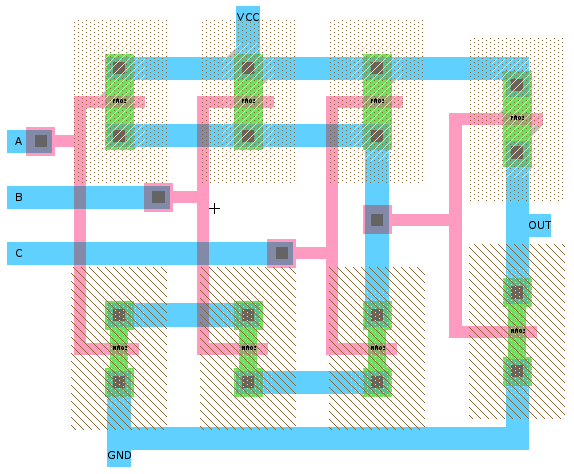
\includegraphics[scale=0.35]{./pics/lay_and_3.png}
      \caption{Layout en electric de la compuerta AND de $3$ entradas.}
	\label{fig1}
\end{figure}
\begin{figure}[H]
  \centering
    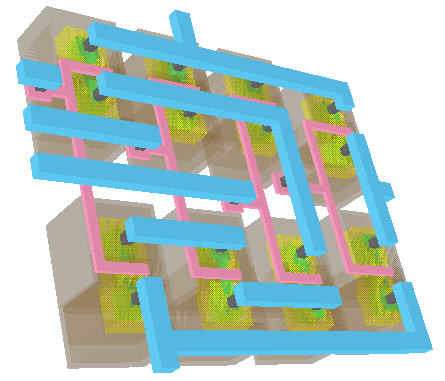
\includegraphics[scale=0.35]{./pics/3d_and_3.png}
      \caption{Layout en electric en $3D$ de la compuerta AND de $3$ entradas.}
	\label{fig2}
\end{figure}
\noindent
Como se puede observar en la Fig.~\ref{fig3} la salida de la compuerta AND con sus $3$ respectivas entradas, en la Fig.~\ref{fig3} se puede observar en verde fosforescente.
\begin{figure}[H]
  \centering
    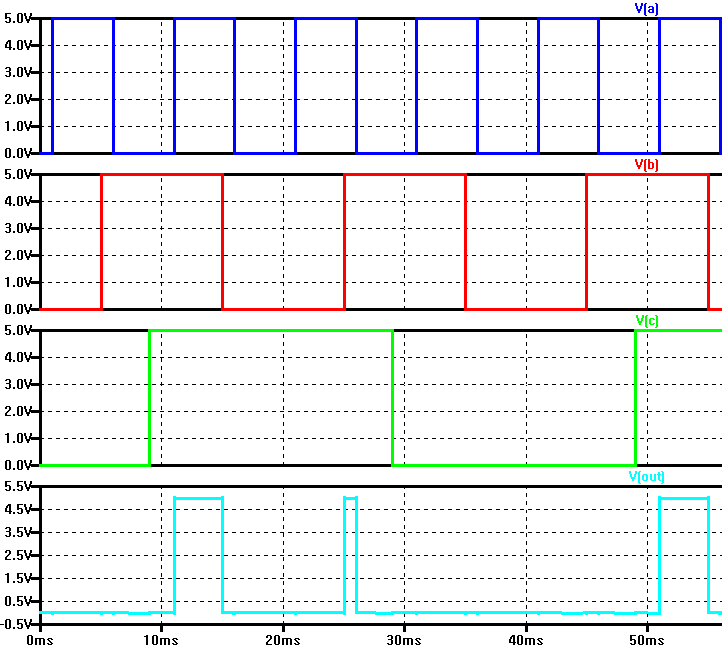
\includegraphics[scale=0.3]{./pics/salida_and_3.png}
      \caption{Simulación en Spice de la AND $3$ entradas implementado.}
	\label{fig3}
\end{figure}
\noindent
Como se puede observar la salida corresponde a la operación AND, solo cuando las $3$ entradas se encuentren en $1$ lógico la salida también sera un $1$ lógico, de lo contrario la salida estará en $0$ lógico.

\section{Diseño flip-flop D}
\noindent
En la fig.~\ref{ffd} se muestra el diagrama esquemático del flip-flop D a implementar, donde el bloque $C$ representa una compuerta de transmisión. Para la elaboración del layout se usó el inversor desarrollado en la práctica pasada, de modo que fue posible insertar varias instancias del módulo.
\begin{figure}[H]
  \centering
    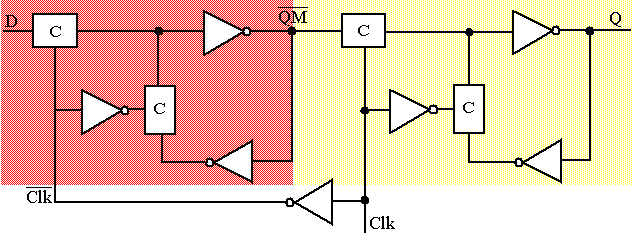
\includegraphics[scale=0.35]{./pics/ffd.png}
      \caption{Esquemático del flip-flop D a implementar.\cite{ff}}
	\label{ffd}
\end{figure}
\noindent
En las fig.~\ref{layoutff}~y~\ref{layoutc} se muestran los layout en \textit{Electric} del flip-flop y de la compuerta de transmisión, correspondientemente.
\begin{figure}[H]
  \centering
    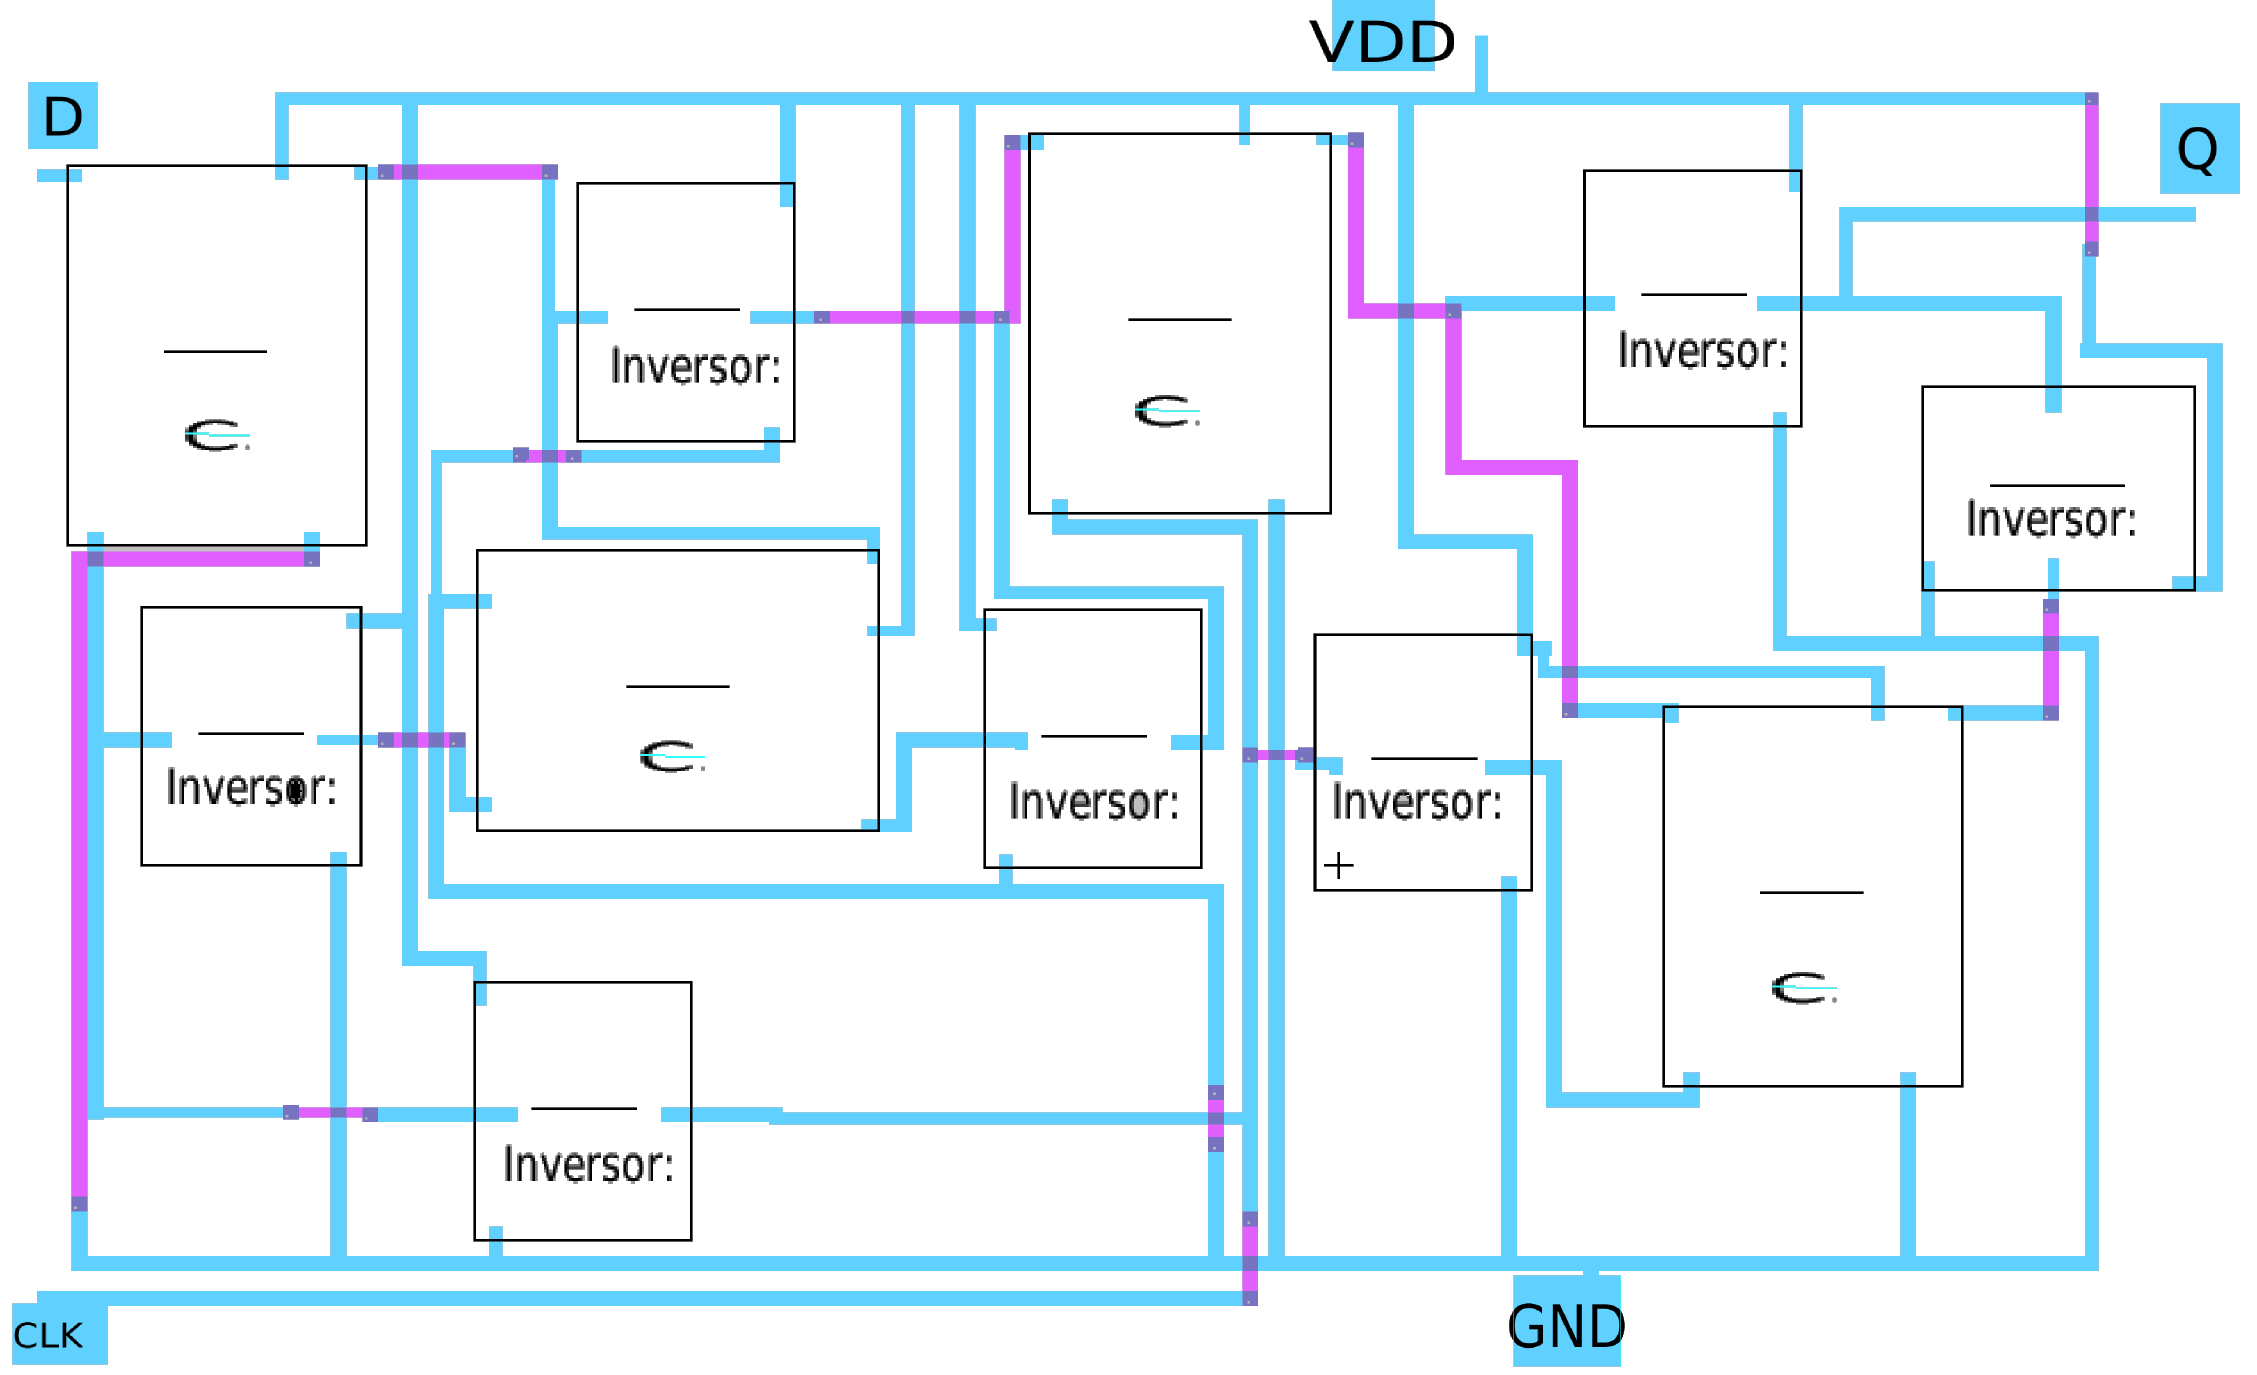
\includegraphics[scale=0.12]{./pics/layoutff2.png}
      \caption{Layout en electric del flip-flop D}
	\label{layoutff}
\end{figure}

\begin{figure}[H]
  \centering
    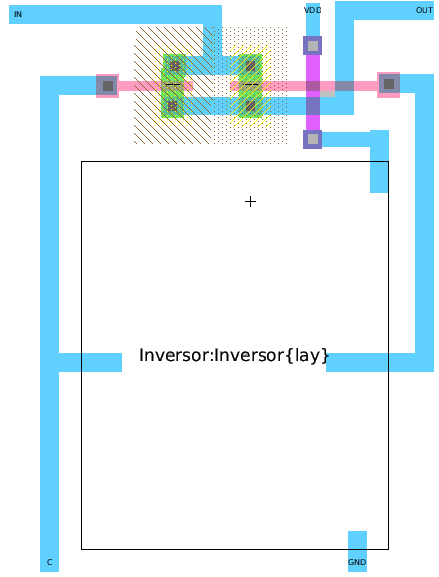
\includegraphics[scale=0.3]{./pics/layoutc.png}
      \caption{Layout en \textit{Electric} de la compuerta de transmisión}
	\label{layoutc}
\end{figure}
\noindent
La salida $Q$ del flip-flop toma el valor de la entrada $D$  únicamente  en los flancos de subida del reloj $Clk$. Por tanto, el flip-flop funciona como un elemento de almacenamiento. La implementación consiste en la unión de dos latches sensibles por nivel: un \textit{master} (color rosa en la fig.~\ref{ffd}) cuya salida $Q_m$ toma el valor de $D$ para niveles bajos del reloj; y un \textit{slave} (color amarillo en la fig.~\ref{ffd}) que toma el valor de $Q_m$ para niveles altos del reloj. De ahí entonces que la salida solo sigue a la entrada en los flancos de subida del reloj. Este comportamiento se ilustra en la fig.~\ref{ffbehavior}.
\begin{figure}[H]
  \centering
    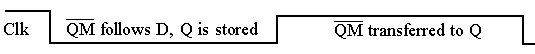
\includegraphics[scale=0.4]{./pics/ffbehavior.png}
      \caption{Descripción del comportamiento de los latches de acuerdo al nivel del reloj $Clk$.}
	\label{ffbehavior}
\end{figure}
\noindent
En la fig.~\ref{ffsim} se muestra la simulación del flip-flop obtenida en Spice. Para $t=15,25,45$ ms, que corresponden a flancos de subida del reloj, se tiene que la señal de salida actualiza su valor acorde a la señal de entrada.
\begin{figure}[H]
  \centering
    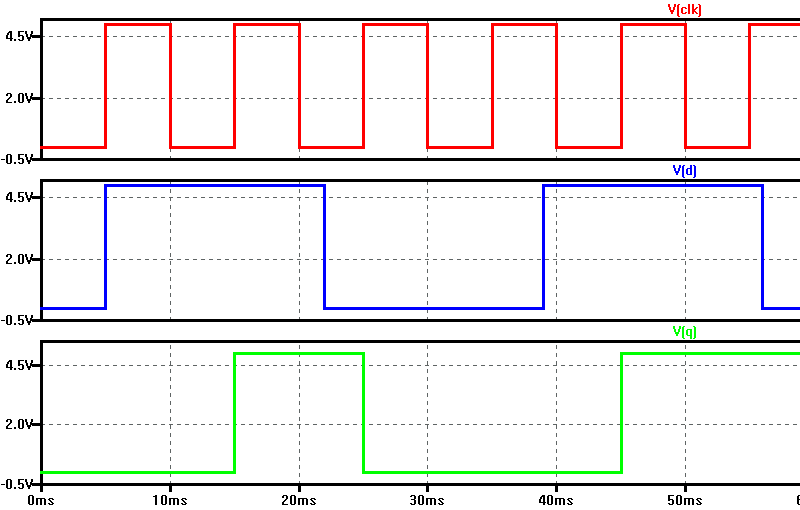
\includegraphics[scale=0.3]{./pics/sim_ff2.png}
      \caption{Simulación en \textit{Spice} del flip-flop implementado.}
	\label{ffsim}
\end{figure}

\subsection{Planteamiento}
\noindent


\section{Análisis de resultados y conclusiones}
\subsection{Compuerta $AND$ de $3$ entradas}
\noindent
Como se puede observar en la Fig.~\ref{fig3} se ha cumplido el objetivo del diseño inicial que era realizar una compuerta AND de $3$ entradas como se vio en ~\ref{AND3} la salida corresponde a la configuración deseada determinada por el diseño inicial. Al momento de invertir la salida de la compuerta NAND de $3$ entradas se optimizan 3 inversores, que si se invierte cada una de las $3$ entradas de la misma compuerta.

\subsection{Diseño flip-flop D}
\noindent


\subsection{Planteamiento}
\noindent


\bibliographystyle{ieeetran}
\begin{thebibliography}{99} 
  \bibitem{ff} The University of New Mexico.
  {\em `Pass Gates Applications: Latches and Registers'}.
  Disponible en \url{http://www.ece.unm.edu/~jimp/vlsi/slides/c1_basics.html}
  
  \bibitem{sedra} Sedra, Adel S. \& Smith, Kenneth C.
  {\em "`Circuitos Microelectrónicos"'}.
  Oxford University Press, Cuarta Edición, 1999.  
\end{thebibliography}
\end{document}